%--------------------------------------------------------------------------------------
% Metodologia a ser empregada 
%--------------------------------------------------------------------------------------
A realização deste trabalho depende do emprego de duas metodologias, uma para o levantamento bibliográfico, etapa qual já foi realizada, e outra para atingir os objetivos almejados pelo trabalho, a ser colocada em prática.
Ambas as metodologias encontram-se descritas a seguir sob os respectivos nomes de: método de pesquisa bibliográfica e método de pesquisa prática.

\textbf{Método de pesquisa bibliogŕafica}

O método de pesquisa bibliográfica consiste num levantamento bibliográfico feito com auxílio do Google Acadêmico \url{https://scholar.google.com.br/} para a pesquisa inicial, sobre os seguintes temas: Recuperação de Informação, Mineração de Textos, Mineração de Dados, Análise de Textos e Classificação de Autores.
Foi utilizada como critério de seleção dos artigos e livros os seguintes pontos:
\begin{itemize}
    \item Estar escrito em português ou inglês; e
    \item Ter no resumo/sumário quaisquer das palavras-chave: Recuperação de Informação; Mineração de Textos; Mineração de Dados, Análise de Textos; Classificação de Autores; Information Retrieval; Text Mining; Data Mining; Text Analysis; e Autor Profiling; e
    \item Disponibilidade gratuita pela internet, podendo ser encontrado utilizando o Google ou Google Scholar ou disponibilizado pela Library Genesis \url{http://gen.lib.rus.ec/} ou Sci-Hub \url{http://sci-hub.tw/}.
\end{itemize}
Artigos e livros mais recentes foram priorizados, assim como aqueles com maior número de citações por outros artigos com os mesmos temas de interesse.

Os artigos e livros foram categorizados de acordo com as cinco palavras chave estabelecidas acima nos critérios do levantamento.
Para seleção dos artigos, o autor realizou uma revisão livre escolhendo aqueles artigos que julgou relevantes, sendo estes lidos em sua totalidade, anotados e resumidos e devidamente fichados. 
Para seleção dos livros, o autor fez uma análise do sumário, localizando os os capítulos pertinentes aos temas do levantamento, e estes então lidos e também resumidos.

O processo de levantamento bibliográfico foi feito interativamente com a escrita da fundamentação teórica para o  trabalho, na qual são abordadas as áreas de e técnicas de RI (Recuperação de Informação) e também as de MT (Mineração de Texto).

\textbf{Método de pesquisa prática}


Para alcançar os objetivos do trabalho, o autor elaborou uma metodologia com o objetivo de avaliar o desempenho dos atributos, gerados a partir da função de ranqueamento BM25, em Mineração de Texto. 
Esta metodologia está ilustrada na Figura \ref{fig:diagrama-da-metodologia} e o processo é detalhado a seguir.
    
    % \begin{figure}[H]
    \begin{center}
    \captionof{figure}{\label{fig:diagrama-da-metodologia} Metodologia proposta para avaliação de desempenho, em verde estão as variáveis mensuráveis sugeridas.}
    
        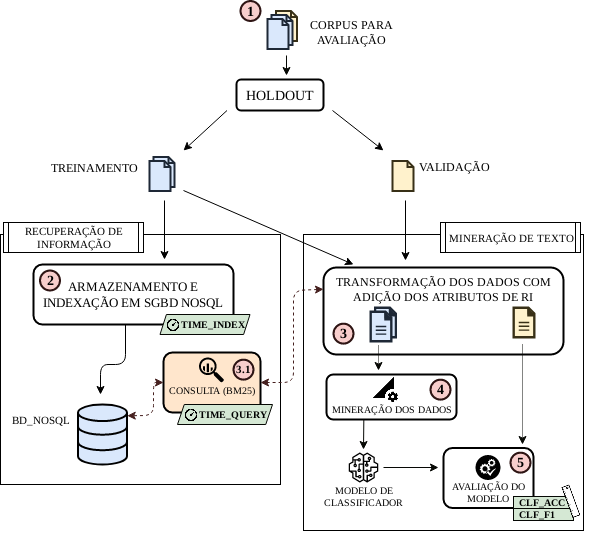
\includegraphics[width=0.8\textwidth]{img/diagrama-metodologia-v2-3.png}
    \end{center}
% \end{figure}
    
    Inicialmente será necessário selecionar os \textbf{(1) Corpus para Avaliação} que servirão para efetuar as avaliações de desempenho, e, caso esses corpus ainda não estejam segmentados em exemplos para treinamento e exemplos para validação, será feita essa separação com o método de \textit{holdout}
    \footnote{Particionamento aleatório do dados em dois conjuntos independentes, geralmente chamados de treinamento e teste. O conjunto de treinamento é utilizado para derivar o modelo e o de teste para estimar a sua acurácia. \cite[p.~370]{Han:2011:DMC:1972541}.} 
    de $\frac{2}{3}$ para treinamento e $\frac{1}{3}$ para validação.
    
    Em seguida, o conjunto de treinamento passará pela fase de RI, aonde será feito o \textbf{(2) Armazenamento e Indexação em  SGBD NoSQL} por meio das ferramentas apresentadas na Seção \ref{sec:Armazenamento-e-indexação}, sendo mensurado o tempo necessário para concluir essa operação em cada um dos Sistemas Gerenciadores de Banco de Dados (SGBD) NoSQL selecionados.
    
    O processo de Mineração de Texto pode ser segmentado em 7 etapas.
    Na metodologia proposta aqui a fase de MT assume que as 3 etapas iniciais de limpeza, integração, e seleção dos dados, já foram realizadas no banco de dados de teste, assim os conjuntos divididos em treinamento e validação passarão diretamente pela etapa seguinte que é a \textbf{(3) Transformação dos dados com adição dos atributos de RI}.
    Nesta etapa, os banco de dados NoSQL indexados receberão \textbf{(3.1) Consultas} com a utilização das funções de ranqueamento baseadas no BM25 que cada ferramenta implementa, sendo mensurado o tempo para efetuar cada consulta e gerar os novos atributos sugeridos adiante na Seção \ref{sec:Atributos-de-RI-sugeridos}.
    
    O processo de \textbf{(4) Mineração dos Dados} será feito por meio da réplica de soluções dos corpus para avaliação selecionados, que possuam seus códigos-fonte disponíveis, sendo então reproduzida cada solução 
    \begin{enumerate*}[label=(\alph*)]
        \item sem nenhuma alteração, e 
        \item com adição dos novos atributos sugeridos.
    \end{enumerate*}
    Esse processo gerará dois modelos de classificador, o primeiro criado sem atributos de RI e o segundo com esses atributos.
    A etapa de \textbf{(5) Avaliação do Modelo} permitirá que para cada modelo sejam geradas medidas da literatura de MT, detalhadas logo mais na Subseção \ref{subsec:Desempenho-de-classificador}, a partir do teste com o conjunto de validação, possibilitando a comparação do ganho de desempenho de classificador com/sem atributos de RI.

\section{Corpus para avaliação}  \label{sec:Corpus-para-avaliação}
    Foram definidos dois corpus de competições promovidas pela PAN, sigla da organização que se originou do \textit{International Workshop on Plagiarism Analysis, Authorship Identification, and Near-Duplicate Detection} em 2007 \cite{PAN_Workshop_2007}, sendo estes descritos a seguir:

    \begin{itemize}
        \item \textbf{DB\_AUTHORPROF - \textit{Author Profiling - PAN @ CLEF 2018}:} Uma tarefa da competição \textit{CLEF 2018} promovida pela PAN na classe de análise de autoria, a qual foca na identificação de gênero no Twitter em três linguagens distintas, inglês, espanhol, e árabe \cite{PAN_APCLEF_2018}.
        
        Os dados consistem de 100 \textit{tweets}
        \footnote{Termo utilizado para designar as publicações feitas na rede social do Twitter.}
         e 10 imagens para cada autor, sendo que o conjunto de treinamento possui \begin{enumerate*}[label=(\alph*)]
            \item 3000 autores em inglês, \item 3000 autores em espanhol, e \item 1500 autores em árabe,
        \end{enumerate*}
        e o conjunto de validação possui
        \begin{enumerate*}[label=(\alph*)]
            \item 1900 autores em inglês, 
            \item 2200 autores em espanhol, e 
            \item 1000 autores em árabe
        \end{enumerate*}
        \cite{rangel2018overview}.
        
        Segundo \citeonline{rangel2018overview} esse banco de dados da \textit{CLEF 2018} com um total de 12600 autores é um subconjunto da tarefa de \textit{Author Profiling} da \textit{CLEF 2017} e eles foram classificados em dois passos,
        \begin{enumerate*}[label=(\roman*)]
            \item automaticamente com a ajuda de um dicionário de nomes próprios, e
            \item manualmente verificando a foto, descrição e outros elementos de cada perfil
        \end{enumerate*}
        \cite{rangel2017overview}.
        
        
        \item \textbf{DB\_HYPARTISAN - \textit{Hyperpartisan News Detection - PAN @ SemEval 2019 Task 4}:} Esta tarefa da competição \textit{SemEval 2019} promovida pela PAN consiste em, dada uma notícia, avaliar se esta segue uma argumentação hiperpartidária, que significa verificar se ela possui fidelidade cega, preconceituosa, ou irracional a um partido, grupo, causa, ou pessoa \cite{PAN_HND_2019}.
        Portanto pode-se dizer que se trata de um problema de classificação binária, a classe real é a presença ou ausência de hiperpartidarismo em cada exemplo.
        
        Os dados consistem em artigos de notícias divididos em múltiplos arquivos onde cada arquivo com parte inicial ``articles-'' consiste em uma notícia e a classificação real da notícia está presente em um arquivo com inicial ``ground-truth-''. 
        Além disso os dados estão divididos em duas partes, a primeira composta de 750 mil artigos está classificada pelo enviesamento geral do editor, onde metade está classificada como hiperpartidária e a outra metade não. 
        Dessa parte, 80\% (600 mil artigos) estão no conjunto de treinamento e 20\% (150 mil) estão no conjunto de validação, sendo que nenhum editor de artigos do conjunto de treinamento se repete no conjunto de validação \cite{johannes_kiesel_2018_1489920}.
        
        A segunda parte dos dados foi rotulada através de \textit{crowdsourcing}
        \footnote{Obter entrada para uma tarefa ou projeto específico contando com os serviços de um número de pessoas, pagas ou não, tipicamente através da Internet.}
        . 
        Essa parte dos dados contêm um total de 645 artigos, sendo estes apenas artigos para os quais existia um consenso entre os trabalhadores de crowdsourcing. 
        Destes, 238 (37\%) são hiperpartidários e 407 (63\%) não são \cite{johannes_kiesel_2018_1489920}. 
    \end{itemize}
    
    Os dois corpus selecionados possuem soluções de participantes nas competições da PAN que tem seu código fonte aberto e disponível em repositórios online.
    Das equipes participantes na competição do corpus DB\_AUTHORPROF, foram localizadas em repositórios de código aberto no GitHub
    \footnote{Plataforma de hospedagem de código-fonte com controle de versão usando o Git.}
     as supostas soluções  apresentadas na Tabela \ref{tab:soluções-authorprof}, ordenadas pela classificação disponível na parte de resultados da página da competição \citeonline{PAN_APCLEF_2018}.    
    
    % \begin{table}[ht]
\begin{center}
    \captionof{table}{\label{tab:soluções-authorprof} Soluções encontradas de participantes da competição DB\_AUTHORPROF.}
    \begin{tabular}{|c|l|l|}
        \hline
        \textbf{Posição}  
        & \makecell[l]{\textbf{Equipe}}
        & \makecell[l]{\textbf{Repositório de código no site \url{https://github.com/}}}
        \\ \hline
        2
        & daneshvar18 
        & \hyperlink{https://github.com/SamanDaneshvar/pan18ap/}{/SamanDaneshvar/pan18ap/}
        \\ \hline
        4
        & laporte18 
        & \hyperlink{https://github.com/arthur-sultan-info/PAN2018-AP/}{/arthur-sultan-info/PAN2018-AP/} 
        \\ \hline
        12
        & gouravdas18 
        & \hyperlink{https://github.com/brajagopalcse/PAN2018/}{/brajagopalcse/PAN2018/}
        \\ \hline
        16
        & schaetti18 
        & \hyperlink{https://github.com/nschaetti/PAN18-Author-Profiling}{/nschaetti/PAN18-Author-Profiling/}
        \\ \hline
        21
        & raiyani18 
        & \hyperlink{https://github.com/kraiyani/author-profiling-pan-clef-2018/}{/kraiyani/author-profiling-pan-clef-2018}
        \\ \hline
        23
        & karlgreen18 
        & \hyperlink{https://github.com/jussikarlgren/pan18}{/jussikarlgren/pan18/}
        \\ \hline
    \end{tabular}
    \legend{\ABNTEXfontereduzida \textbf{Fonte:} Classificações obtidas de \citeonline{PAN_APCLEF_2018}, e repositórios encontrados pelo autor.}
\end{center}
% \end{table}

    Quanto à competição referente ao corpus DB\_HYPARTISAN foram encontrados os repositórios disponíveis na ordem de classificação da página da competição \cite{PAN_HND_2019}, dispostos abaixo na Tabela \ref{tab:soluções-hyperpartisan}.
    
    % \begin{table}[ht]
\begin{center}
    \captionof{table}{\label{tab:soluções-hyperpartisan} Soluções encontradas de participantes da competição DB\_HYPERPARTISAN.}
    \begin{adjustbox}{max width={\textwidth},keepaspectratio}%
    \begin{tabular}{|c|l|l|}
        \hline
        \textbf{Posição}  
        & \makecell[l]{\textbf{Equipe}}
        & \makecell[l]{\textbf{Repositório de código no site \url{https://github.com/}}}
        \\ \hline
        1
        & bertha-von-suttner 
        & \hyperlink{https://github.com/GateNLP/semeval2019-hyperpartisan-bertha-von-suttner/}{/GateNLP/semeval2019-hyperpartisan-bertha-von-suttner/}
        \\ \hline
        4
        & tom-jumbo-grumbo 
        & \hyperlink{https://github.com/chialun-yeh/SemEval2019/}{/chialun-yeh/SemEval2019/} 
        \\ \hline
        10
        & clint-buchanan 
        & \hyperlink{https://github.com/hmc-cs159-fall2018/final-project-team-mvp-10000/}{/hmc-cs159-fall2018/final-project-team-mvp-10000/}
        \\ \hline
        13
        & paparazzo 
        & \hyperlink{https://github.com/ngannlt/semeval2019-hyperpartisan-paparazzo/}{/ngannlt/semeval2019-hyperpartisan-paparazzo/}
        \\ \hline
        17
        & spider-jerusalem 
        & \hyperlink{https://github.com/amal994/hyperpartisan-detection-task/}{/amal994/hyperpartisan-detection-task/}
        \\ \hline
        19
        & doris-martin 
        & \hyperlink{https://github.com/ixa-ehu/ixa-pipe-doc/}{/ixa-ehu/ixa-pipe-doc/}
        \\ \hline
    \end{tabular}
    \end{adjustbox}
    \legend{\ABNTEXfontereduzida \textbf{Fonte:} \cite{PAN_HNDLEADERBOARD_2019}.}
\end{center}
% \end{table}

    As soluções com código fonte encontradas serão analisadas para garantir que já não façam uso da criação de atributos baseados em RI.
    Então, no mínimo uma solução de cada BD será executada para verificação das pontuações obtidas na competição e obtenção das medidas de desempenho de classificador (ver a Subseção \ref{subsec:Desempenho-de-classificador}).
    Em seguida, será executado o processo completo da metodologia apresentada na Figura \ref{fig:diagrama-da-metodologia}, para mensurar o desempenho computacional das ferramentas de armazenamento e indexação, e o desempenho do classificador com os atributos de RI.
    
    
\section{Armazenamento e indexação} \label{sec:Armazenamento-e-indexação}

    Para armazenar e indexar os corpus das tarefas de Mineração de Textos em bancos de dados, possibilitando o cálculo da função BM25 para que sejam gerados os atributos sugeridos na Seção \ref{sec:Atributos-de-RI-sugeridos} para cada exemplo, serão utilizadas as seguintes tecnologias que fazem implementações do BM25:
    \begin{itemize}
        \item \textbf{TOOL\_ELASTIC}: Elasticsearch 7.2 é o mecanismo distribuído de análise e busca baseado no Apache Lucene\footnote{Biblioteca de software livre e de código aberto para ferramentas de buscas em texto, escrita originalmente em Java \cite{LUCENE_DOCUMENTATION_2019}.}, desenvolvido em Java, e possui código aberto sob diversas licenças sendo a principal a Licença Apache
        \footnote{Licença de software livre permissiva de autoria da Apache Software Foundation (ASF) \cite{NEWMEDIA_OPENGUIDE_2015}.}
         \cite{ELASTIC_REFERENCE_INTRO_2019}. 
        
        O Elasticsearch possui diversas APIs que possibilitam sua integração fácil com variadas linguagens de programação, e tenta deixar todas suas funcionalidades disponíveis via sua API JSON pois internamente é no formato JSON
        \footnote{\textit{JavaScript Object Notation}, formato de objeto utilizado pela linguagem de programação JavaScript.}
         que o Elasticsearch guarda os dados. 
        Suporta também requisições GET em tempo real, o que o torna apropriado para armazenamento como um banco de dados NoSQL \cite{PETER_ELASTICDB_2011, VOLKAN_ELASTIC_DATASTORE_2018}.
        
        Dentre suas funções de indexação, o Elasticsearch possui um módulo de similaridade (\textit{similarity module}) que é responsável pela implantação de funções para ranqueamento de documentos.
        Este módulo realiza uma implementação da função BM25 como sua função padrão para cálculo de similaridade sobre o nome de \textit{BM25 similarity} \cite{ELASTIC_REFERENCE_SIMILARITY_2019}.
        
        \item \textbf{TOOL\_ARANGO}: ArangoDB v3.4.6 é um banco de dados multi-modelo nativo, desenvolvido principalmente em C++ com extensões em JavaScript, e possibilita modelos de dados flexíveis, tanto para documentos, gráficos, e valores-chave \cite{ARANGODB_DOC_2019}.
        
        Utiliza da linguagem de consulta AQL (\textit{ArangoDB Query Language}) para recuperar e modificar dados, que, por meio das \textit{views}
        \footnote{``Uma \textit{view} (visão) em terminologia SQL é uma única tabela que é derivada de outras tabelas [$\cdots$]  é considerada uma tabela virtual'' \cite[p.~88]{ElmasriSBD2010}.}
         do tipo arangosearch, introduz uma camada de integração com a biblioteca IResearch
        \footnote{Biblioteca de mecanismo de busca orientada a documentos, multiplataforma, e de alto desempenho, escrita inteiramente em C++, com o foco em uma conectividade de diferentes modelos de ranqueamento/similaridade \cite{IRESEARCH_GITHUB_2019}.}
        .
        Assim, por meio da AQL integrada ao IResearch, o ArangoDB fornece funções de ordenação de documentos mediante uma consulta, e, dentre elas, a função BM25() faz uma implementação do algoritmo da função de ranqueamento BM25 \cite{ARANGODB_SEARCHVIEWS_2019}.
        
        \item \textbf{TOOL\_ZETTAIR}: Zettair v0.9.3 é um mecanismo de busca de código-fonte aberto escrito na linguagem C, desenvolvido pelo Grupo de Mecanismos de Busca do Instituto Real de Tecnologia de Melbourne em 2009 \cite{ZETTAIR_HOME_2009}.

        O Zettair permite que coleções no formato HTML ou TREC sejam indexadas para busca, e possui como característica principal a habilidade de lidar com grandes quantidades de texto, ele constrói índices invertidos por meio da análise feita no seu modo de construção de índex \cite{ZETTAIR_INDEX_2009}.
        
        Os arquivos de índices invertidos construídos pelo Zettair podem então ser consultados utilizando duas medidas diferentes \cite{ZETTAIR_USAGE_2009}:
        \begin{itemize}
            \item \textbf{--cosine}: Uma implementação da medida da similaridade do cosseno; e
            
            \item \textbf{--okapi}: Implementação da função BM25, também chamada de Okapi BM25.
        \end{itemize}
    \end{itemize}

\section{Atributos de RI sugeridos}  \label{sec:Atributos-de-RI-sugeridos}
    Os atributos baseados em Recuperação de Informação sugeridos para a presente pesquisa são fundamentados na investigação de \citeonline{WEREN_MESTRADO_2014}, derivada de seus trabalhos anteriores \cite{WEREN_CLEF_2014,WEREN_ARTIGO_2014}, os quais mostram resultados positivos da utilização de atributos derivados de RI numa tarefa de Mineração de Texto.
    Nesses trabalhos, para identificação de perfis de autoria, são utilizados grupos de atributos derivados de RI, os quais representam a seguinte hipótese: os autores de um mesmo grupo de gênero ou idade tendem a usar termos semelhantes, e que a distribuição desses termos difere entre os grupos \cite[p.~20]{WEREN_MESTRADO_2014}.
    
    Esse mesmo pressuposto, da investigação feita por \citeonline{WEREN_MESTRADO_2014}, é assumido aqui, sendo generalizado para outras classes de identificação de autoria, como por exemplo que autores de artigos hiperpartidários tendem a usar termos semelhantes, e a distribuição desses termos difere de autores não hiperpartidários.
    
    % \begin{figure}[H]
    \begin{center}
    \captionof{figure}{\label{fig:diagrama-cosulta-geração-atributos} Metodologia de consulta aos BD para geração dos atributos sugeridos, exemplificação da lista de resultados para uma única consulta.}
        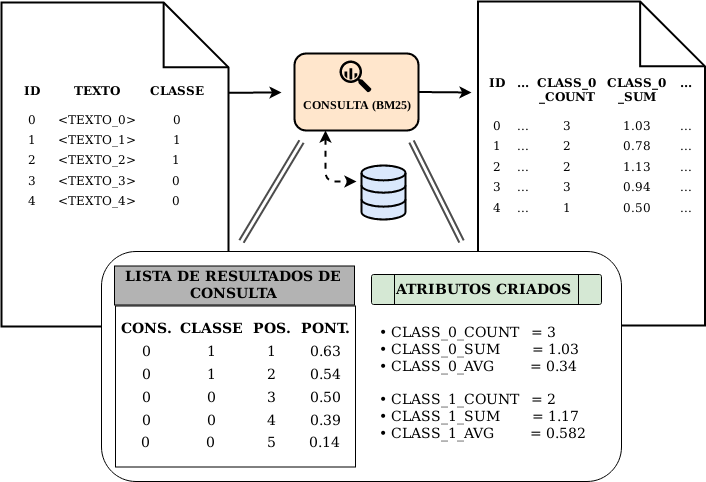
\includegraphics[width=0.8\textwidth]{img/diagrama-consulta-geracao-atributo.png}
\end{center}
% \end{figure}
    
    Cada exemplo do corpus a ser classificado será usado como consulta ao banco de dados NoSQL indexado, e cada uma destas consultas terá como resultado uma lista dos \textit{top-$k$} exemplos presentes no banco de dados, ordenada por pontuação de similaridade da função BM25, sendo esta pontuação calculada pela ferramenta de armazenamento indexação. Este procedimento está representado na Figura \ref{fig:diagrama-cosulta-geração-atributos}.
    
    O cálculo dos novos atributos será feito a partir da lista retornada dos \textit{top-$k$} exemplos, onde serão utilizadas as três funções de agregação sugeridas por \citeonline[p.~21--23]{WEREN_MESTRADO_2014}:
    \begin{enumerate*}[label=(\alph*)]
        \item média,
        \item soma, e
        \item contagem
    \end{enumerate*}, 
    levando em conta a classe binária da tarefa de classificação. 
    Assim, serão gerados os atributos apresentados na Tabela \ref{tab:lista-atributos-sugeridos}.
    
    % \begin{table}[H]
\begin{center}
    \captionof{table}{\label{tab:lista-atributos-sugeridos} Atributos derivados de RI sugeridos.}
    \begin{adjustbox}{max width={\textwidth},keepaspectratio}%
    \begin{tabular}{|p{4.0cm}|p{4.5cm}|p{4.5cm}|}
        \hline
        \diagbox[width=4.4cm, height=2.0cm]{Agregação}{
            \raisebox{-1.3cm}{
                \rotatebox{90}{
                    \parbox{1.5cm}{\centering Exemplo}
                }
            }
        }  
        & \makecell[l]{\parbox{4.0cm}{Não faz parte da \\ classe da tarefa}}
        & \makecell[l]{\parbox{4.0cm}{Faz parte da \\ classe da tarefa}}
        \\ \hline
        \makecell[l]{Média aritmética \\ das pontuações}
        & \textbf{CLASS\_0\_BM25\_AVG} 
        & \textbf{CLASS\_1\_BM25\_AVG}  
        \\ \hline
        \makecell[l]{Contagem do número \\ de resultados}
        & \textbf{CLASS\_0\_BM25\_COUNT} 
        & \textbf{CLASS\_1\_BM25\_COUNT}  
        \\ \hline
        \makecell[l]{Soma das \\ pontuações}
        & \textbf{CLASS\_0\_BM25\_SUM} 
        & \textbf{CLASS\_1\_BM25\_SUM}  
        \\ 
        \hline
    \end{tabular}%
    \end{adjustbox}%
    \legend{\ABNTEXfontereduzida \textbf{Fonte:} O autor.}
\end{center}
% \end{table}

\section{Medidas para avaliação de desempenho}  \label{sec:Medidas-para-avaliação-de-desempenho}
    Serão avaliados
    \begin{enumerate*}[label=(\alph*)]
        \item o desempenho das ferramentas utilizadas para indexação e consulta, por meio da avaliação temporal do desempenho computacional, e também
        \item o ganho de desempenho propiciado pelo uso dos atributos de RI em termos das medidas de classificadores de Mineração de Texto. 
    \end{enumerate*} 
    
    \subsection{Desempenho computacional das ferramentas}  \label{subsec:Desempenho-computacional}
        Para avaliar o desempenho das ferramentas de armazenamento e indexação serão utilizadas duas medidas temporais:
        \begin{itemize}
            \item \textbf{TIME\_INDEX}: Tempo de execução para indexar o conjunto de treinamento de cada um dos corpus para avaliação elencados na Seção \ref{sec:Corpus-para-avaliação}. Dadas as quatro diferentes ferramentas de indexação e os dois corpus selecionados, serão computadas 8 TIME\_INDEX para comparação;
            
            \item \textbf{TIME\_QUERY}: Tempo para consulta de cada exemplo do conjunto de teste e geração dos atributos sugeridos na Seção \ref{sec:Atributos-de-RI-sugeridos} para o item específico. Dadas os 12 atributos sugeridos para criação distribuídas nos dois banco de dados selecionados, e dadas as 4 ferramentas de indexação, 48 TIME\_QUERY serão computadas.  
        \end{itemize}
        
        Essas variáveis serão computadas para cada uma das 4 ferramentas selecionadas sendo executadas no mesmo sistema computacional a fim de oferecer maior confiança aos números obtidos. 
        O sistema computacional a ser utilizado para efetuar o experimento ainda não está definido, mas será especificado nos resultados.
    
    \subsection{Desempenho de classificador}  \label{subsec:Desempenho-de-classificador}
        O ganho de desempenho propiciado pelos atributos de RI criados será mensurado por medidas de desempenho de classificadores da literatura de mineração de dados, as mesmas também utilizadas na Mineração de Texto.

        % \begin{minipage}{.5\textwidth}
            \begin{equation}
                \label{eq:medida-acurácia}
        		acc = 
        		\frac{\textit{TP} + \textit{TN}}{P + N}
            \end{equation}
        % \end{minipage}

        Nesse estudo serão computadas as seguintes medidas:
        \begin{itemize}
            \item \textbf{CLF\_ACC}: Acurácia do classificador no conjunto de validação.
            \item \textbf{CLF\_F1}: $F_1$-score do classificador no conjunto de validação.
        \end{itemize}
        A acurácia de um classificador, definida pela Equação \ref{eq:medida-acurácia}, é a razão entre o número de exemplos classificados corretamente, e o número total de exemplos, no caso em questão, a variável \textbf{CLF\_ACC} a ser computada é referente ao conjunto de validação.

        % \noindent\begin{minipage}{.5\textwidth}
            \begin{equation}
                \label{eq:medida-f-score}
        		F = 
        		\frac{2 \times p \times r}{p + r}
            \end{equation}
        % \end{minipage}

        O $F_1$-score é uma medida de classificador que engloba a precisão e revocação (ou sensitividade), e também é uma boa medida da efetividade de classificadores em termos comparação pois engloba mais informação do que a acurácia. 
        É calculado conforme a definição dada pela Equação \ref{eq:medida-f-score}.

        \noindent\begin{minipage}{.5\textwidth}
        \end{minipage}
        